\begin{figure}
    \centering
    \resizebox{!}{.8\textheight}{
        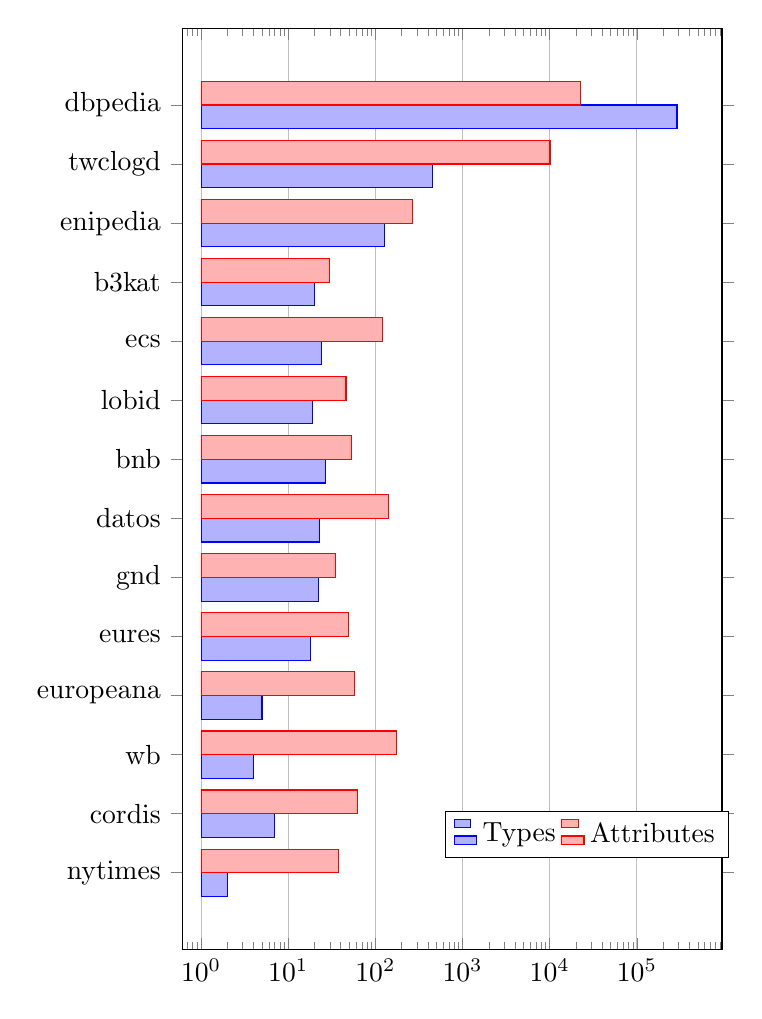
\begin{tikzpicture}[remember picture]
            \begin{axis}[
                    xbar=0pt,
                    y=.75cm,
                    symbolic y coords={nytimes,cordis,wb,europeana,eures,gnd,datos,bnb,lobid,ecs,b3kat,enipedia,twclogd,dbpedia},
                    bar width=0.3cm,
                    ytick=data,
                    xmode = log,
                    xmajorgrids = true,
                    legend style={at={(0.75,0.15)}, anchor=north,legend columns=-1},
                ]
                \addplot coordinates { (2,nytimes) (7,cordis) (4,wb) (5,europeana) (18,eures) (22,gnd) (23,datos) (27,bnb) (19,lobid) (24,ecs) (20,b3kat) (128,enipedia) (450,twclogd) (288524,dbpedia) };
                \addplot coordinates { (38,nytimes) (63,cordis) (174,wb) (58,europeana) (49,eures) (35,gnd) (143,datos) (53,bnb) (46,lobid) (120,ecs) (30,b3kat) (267,enipedia) (10060,twclogd) (22369,dbpedia) };
                \legend{Types,Attributes}
            \end{axis}
        \end{tikzpicture}
    }
\end{figure}
%% vim: et:sw=4
